% thesis.tex
%
% requirements
%   jsclasses
%   thesis.sty
%

%% JISフォントメトリックが用意されていない場合(debian等)は,
%% 従来のmingothを用いる.
%\documentclass[mingoth,11pt,openany,a4paper]{jsbook}
%% 標準
%% openanyを省くと,右側のページから章がはじまる
	
% pdf用の文書情報
\input docinfo.out

\documentclass[12pt,a4paper]{jsbook}

\usepackage{graphicx}

\usepackage{bm}
\usepackage{amscd}
\usepackage{amssymb}
\usepackage{amsfonts}
\usepackage{multicol}
\usepackage{amsmath}
\usepackage{array}
\usepackage{subfigure}
\usepackage{setspace}

\graphicspath{{./figurtes/}}

% TXフォントを使う
\usepackage{txfonts}

% 独自論文スタイルの使用
\usepackage{thesis}

% for dvipdfm
\usepackage[dvipdfmx]{color}
%\usepackage[dvipdfmx,bookmarks=true,bookmarksnumbered=true,bookmarkstype=toc,%
%    pdftitle=\PDFTITLE, %
%    pdfsubject=\PDFSUBJECT, %
%    pdfauthor=\PDFAUTHOR, %
%    pdfkeywords=\PDFKEYWORDS]{hyperref}
%\ifnum 42146=\euc"A4 \AtBeginDvi{\special{pdf:tounicode EUC-UCS2}}\else
%\AtBeginDvi{\special{pdf:tounicode 90ms-RKSJ-UCS2}}\fi

% 一行の文字制限(40zw)をなくす
\setlength{\textwidth}{\fullwidth}
\renewcommand{\baselinestretch}{1.1}
\setcounter{tocdepth}{2}

% evensidemarginの再定義
% この部分は jsbook.cls の定義と同じです.
% jsbook.cls の定義がかわっていれば,そちらにあわせて下さい.
\setlength{\evensidemargin}{\oddsidemargin}
\addtolength{\evensidemargin}{\fullwidth}
\addtolength{\evensidemargin}{-\textwidth}

% とじしろの確保
% defaultではとじしろがないので,その分ずらします.
\addtolength{\oddsidemargin}{8mm}
\addtolength{\evensidemargin}{-8mm}

% \renewcommand{\baselinestretch}{1.38}
% \kanjiskip=.1zw plus 3pt minus 3pt
% \xkanjiskip=.1zw plus 3pt minus 3pt

% \makeatletter
% \renewcommand{\theequation}{\thesection.\arabic{equation}}
% \@addtoreset{equation}{section}

% \renewcommand{\thetable}{\thesection.\arabic{table}dn}
% \@addtoreset{table}{section}

% \renewcommand{\thefigure}{\thesection.\arabic{figure}}
% \@addtoreset{figure}{section}

% \renewcommand{\paragraph}{\@startsection{paragraph}{4}{\z@}%
%    {1.5\Cvs \@plus.5\Cdp \@minus.2\Cdp}%
%    {.5\Cvs \@plus.3\Cdp}%
%    {\reset@font\normalsize\bfseries}}
%    
% \makeatother

\DeclareMathOperator{\sgn}{sgn}

\frontmatter

% thesis(論文の区別),title(題),date(提出日),teacher(指導教官),
% organization(所属), author(著者), \idnumber(学生証番号)

\thesis{修士学位論文} 
\title{表面構造を考慮した\\複眼のリアルタイムレンダリング}
% \engtitle{Detailed Surface Representation of Fluid by Multi-scale Simulation}
\organization{東京大学大学院 学際情報学府}
\course{先端表現情報学コース} %%所属
\date{平成26年度}
\author{佐川 和輝}
\teacher{河口 洋一郎 教授}
\idnumber{136313}

\begin{document}

% 表紙
\maketitle
\begin{spacing}{1.5}
%\include{abstract}

% 目次
\thispagestyle{headings}
\tableofcontents

% 図一覧
\thispagestyle{headings}
\listoffigures

%表一覧
\thispagestyle{headings}
\listoftables

\mainmatter

%\chapter{*タイトル*}
\label{*Ltitle*}

タイトルの中身だよ。

\subsection{サブセクション}
\label{*Lsubsection*}

サブセクション\cite{*AuthorName*}の中身だよ。\figref{test} %画像番号。(Fig1.1)など



\begin{itemize}
\item アイテム1
\item アイテム2
\item アイテム3。文章に出来るよ
\end{itemize}

\begin{figure}[h]
  \centering
  
\includegraphics[width=3.0in]{./img/TEMP}
  \caption{キャプションだよ}{行を変えられるみたい}
  \label{test} %ここで画像のラベリング?
\end{figure}
 
        %テンプレート
\chapter{序論}
\label{CBegin}

\section{研究背景}
\label{SBackground}

コンピュータグラフィックス(Computer Graphics: CG)は、ハードウェアの発展や高性能コンピュータの普及により、近年ではさらに身近なものになっている。
実物と見間違うほどのCGも珍しくなくなり、聴衆は実物とCGとの差異に敏感になってきている。
CG技術の発展により、コンピュータによって作成された画像に対して実写並みのリアリズムが要求されるようになってきた。
CGの歴史上においても、人間が現実世界で目にするものをそのままコンピュータ上に再現することが当初からの目標とされており、一部では実物とCGとの差異が埋まりつつあると言える。

成熟期に入ったとも考えられるCG技術ではあるが、リアリズムの追求はとどまるところを知らず、さらなる技術向上が目指されている。
また、現実世界にはCGによって十分に再現されていないさまざまな光学的な現象が依然として存在することも事実である。
そのため、多くの研究者たちがCGの表現力をさらに向上させるために研究・開発を行っている。


\subsection{体積や厚みを考慮したコンピュータグラフィックス}
\label{SSVolumerendering}

CGは物体やものがどのように「見えるか」をコンピュータによって作成するために生み出された技術である。
そのため、「ものの見た目」においてもっとも重要である物体表面での光の反射がまず取り扱われる。
しかしながら、実際には臓器などの不透明な物体や煙や炎などといった粒子で満たされた一定の領域や体積を考慮する必要のある対象も存在する。
こうした対象を視覚化(visualize:ビジュアライズ)するためには、物体内部や粒子で満たされた領域内部を通過することによって光の挙動にどのような影響が及ぼされるかについても考慮する必要がある。

たとえば、ボリュームレンダリング(Volume Rendering)の手法では、空間をボクセル(voxel)と呼ばれる六面体に分割し、遮る光の量を計算する。
ボクセルごとの密度も考慮しており、密度の大きなボクセルほど多くの光の量を遮る。
歴史的には、医療の分野で用いられるCT(Computed Tomography)データのビジュアライゼーションを目的とする視覚化手法の研究が重ねられていたが、1980年代にCGの分野でもボクセルを用いたボリュームデータの視覚化が行われるようになった。\cite{}
ボリュームレンダリングは主に肉や骨、脂肪といった密度の違う領域をあわせ持つ人体の視覚化する方法として研究が始められたようである。

ほかには、パーティシペイティングメディア(participating media)という自然科学の分野における考え方を導入した手法がある。
煙や炎などは光が物体内部で吸収や散乱を起こしやすく、こうした光の吸収度や散乱度が非常に大きい領域はパーティシペイティングメディアと呼ばれる。
パーティシペイティングメディアをレンダリングするための技法はボリュームレンダリングの技法とともにボリュームをレンダリングするための技法として、CGの歴史上でほぼ同時期に登場した\cite{}。

大理石や人体の皮膚といった半透明の材質をレンダリングするための技法として、サブサーフェイススキャッタリング(subsurface scattering)を考慮した手法も研究が盛んに行われている。
サブサーフェイススキャッタリングとは、一度物体内部に進入した光が物体内部で反射を繰り返し、光が入射した位置とは別の位置から外部へ向かって出射する光の挙動のことである。
自然界のほとんどの物体でこの現象が見られ、半透明の質感を持った大理石や皮膚などにおいて顕著に現れる。
サブサーフェイススキャッタリングを物理的に正確にレンダリングするためには非常に大きな計算不可がかかっていたものの、映画などでのフォトリアリスティックな表現への要求から研究が進み、現在ではすでに実時間での計算手法も開発されている\cite{jorge jimenez}。

以上のように、光が物体内部を通過するオブジェクトのレンダリングに関しては以前から研究が進んでおり成果を上げている。
しかし、いずれも物質レベルのミクロな構造に対する光の挙動を再現したものであり、ミドルレベルの大きさの構造体が集合した物体に対する光の挙動までは扱っていない。

\subsection{生物発想のコンピュータグラフィックス}

人間を対象としたCG表現に関しては数多くの研究がなされているが、人間以外にも動物や昆虫といったさまざまな生物のもつ光学現象を対象としたCG研究も近年では行われるようになってきている。
生物の発する体色などの色は発色のしくみが解明されていないものもあり、たとえば構造色といった表面微細構造によって色が変化するものも存在する。
構造色は光の散乱、回折、干渉などのさまざまな光学現象によって生じる色であり、物体表面の膜構造や回折格子構造などに由来する。
そのため、通常の色素による発色とは異なり、角度や媒質などの観測条件によって色が変化するものが多い。
自然界ではコガネムシやモルフォチョウの翅などの昆虫の体色や孔雀の羽根などが該当する。
現在盛んに行われている物理学をCGに応用した研究と比較して、生物のモーションや体色などの生物学をCGに応用した研究にはまだ手がつけられていない分野も多いため、今後の発展が期待される。

%% \begin{figure}[hn]
%%   \centering
%%   
\includegraphics[width=3.0in]{./img/TEMP}
%%   \caption{構造色の例}
%%   \label{F}
%% \end{figure}

\subsection{リアルタイムでのハイクオリティレンダリング}

近年ではコンピュータ・ハードウェアの高速化により、リアルタイム(real-time:実時間)におけるCG映像の表現力が飛躍的に向上している。
リアルタイムで実写に迫る表現も可能になりつつあり、今後もその要求は高まると考えられる。
\textcolor{red}{********}

\subsection{複眼と偽瞳孔}
\label{SSCompoundeyeandpseudopupil}

複雑な内部構造を有し、さらに生物に関連するものとして昆虫や甲殻類などの複眼が挙げられる。
複眼は個眼と呼ばれる小さな眼の集合体であり、それぞれの個眼にはレンズや色素細胞といったの光学現象に影響する部位が備わっている。
複眼の見た目に関係する光学的な現象として偽瞳孔と呼ばれる現象がある。
偽瞳孔とは複眼表面に現れる黒い斑点模様であり、個眼のレンズによる光の屈折作用と密接に関わっている。

複眼を構成する個眼の数は非常に多く、さらに表面の構造が非常に複雑で細かいためコンピュータで精巧な形状を作成するのは現実的ではない。
また、精巧な形状のみを擬似的に表現する手法はCGにおいても研究が進んでおり、非常に高い効果を上げている。
例を挙げると、ディスプレイスメントマッピングやバンプマッピングなどの手法では、ポリゴン表面に変位情報や法線情報を付加するによって複雑で細かい表面形状を少ない計算量で表現することを可能にしている\figref{}\figref{}。
現在ではアートやエンターテイメントの分野において昆虫の複眼を表現する際にこれらの手法を利用するのが一般的となっている\figref{}。
しかしながら、上記の手法では複眼の表面的な形状を再現するのみにとどまっており、複眼の内部構造を考慮した光学的現象を再現するまでには至っていない。
すなわち、先述の偽瞳孔をCGを用いて再現するための手法は未発展であると言える。

%% \begin{figure}[hn]
%%   \centering
%%   
\includegraphics[width=3.0in]{./img/TEMP}
%%   \caption{ディスプレイスメントマッピング}
%%   \label{F}
%% \end{figure}

%可能なら先生の画像を使わせてもらう

%% \begin{figure}[hn]
%%   \centering
%%   
\includegraphics[width=3.0in]{./img/TEMP}
%%   \caption{バンプマッピング}
%%   \label{F}
%% \end{figure}

\section{本研究の目的}
\label{SObjective}

これまでに紹介したように、技術の進歩にともなって、コンピュータグラフィックスに対する要求は増してきつつある。
さらに、今後はリアルタイムレンダリングにおいても高精細で写実的な表現が求められると考えられる。
\secref{SSVolumerendering}で述べたように、物体内部を通過する光を考察したレンダリング(rendering)手法が生み出されてはいるものの、より複雑で光の挙動に影響を与えるような内部構造を持つ物体のレンダリングに関しては対象ごとに個別の手法を考案する必要がある。
本研究では、昆虫などの複眼表面に現れる光学現象として\secref{SSCompoundeyeandpseudopupil}で述べた偽瞳孔に着目し、この現象のCGによるリアルタイムでの表現手法の研究および開発を目的とする。

\section{本論文の構成}
\label{SPaper_structure}

本論文の構成について述べる。
次の\chapref{CRelatedWork}では、本研究と関連のある技術手法や生物分野で複眼について調査等を行った研究を紹介する。
\chapref{CKnowledge}では、周辺技術として本研究の基礎となるシェーダアルゴリズムについて解説を行う。
続いて\chapref{CExperiment}では、過去の研究を踏まえて本研究で実際に行った予備実験について説明する。
実験結果を踏まえて\chapref{CMethod}では、本研究で提案するシミュレーション手法を述べる。
\textcolor{red}{********}
	%1章 序論
\chapter{関連研究}
\label{CRelatedWork}

りれーてっどわーく。
てすとてすとてすとテストテストテストテストテストテストテストテストテストテストテストテストテストテストテストテスト

\section{微細構造を扱った研究}
\label{SMicrostructure}

表面微細構造をもつ物質をレンダリングする研究が過去にいくつか行われている。


\section{本研究の位置づけ}
\label{SPosition}

本研究の位置づけについて述べる。
		%2章 関連研究
\chapter{複眼の光学的特徴}
\label{CKnowledge}

本章では、昆虫や甲殻類に見られる複眼に関する知識や研究を紹介する。

\section{複眼の性質}

複眼は個眼と呼ばれる単位の視覚器官から構成される\figref{}。
ひとつの個眼にはレンズと光受容細胞(photoreceptor cell)および色素細胞(pigment cell)などが含まれる。
一般に、複眼を構成する個眼の数は複眼の大きさに比例し、ハエなどの少ないものでは数百個、トンボなどの多いものでは2万個以上であると言われている\cite{arikawa-zougan}。

八木\cite{yagi1951studies}によると、昆虫に見られる複眼には複数のタイプがあり、真円錐眼(eucone eye)、偽円錐眼(pseudocone eye)、無円錐眼(acone eye)、外円錐眼(exocone eye)の4種類に大別される。
真円錐眼は堅いキチン質の円錐晶体をもち、独特な光学的性質を有している。
偽円錐眼は流動体もしくは半流動体で満たされたカプセルから構成され、比較的弱い屈折力しか持ち合わせていない。
無円錐眼は円錐晶体を有しておらず、外円錐眼では円錐晶体が角膜面のくぼみによって置き換えられている。
真円錐眼はさらに連立像眼\figref{FRenritsu}と重複像眼\figref{FTyoufuku}に分けられる。

\subsection{連立像眼}

チョウなどの眼は連立像眼(apposition eye)と呼ばれ、昼行性の種に多く見られる。
感覚神経のユニットは円錐晶体の頂点から離れ、ひとつずつ独立して光を受容するような構造になっている\cite{arikawa-zougan}。
すなわち、ひとつひとつの個眼は光学的に独立しており、レンズ直下の感桿に導かれた光は外に漏れることなく感桿基部まで到達する。
Nilsson\cite{}によると連立像眼はさらに少なくとも4タイプに分類され、単純連立型、無限焦点型(afocal type)、分散感桿型(open rhabdom)・神経重複型(nural superposition)、透明連立型などがある。
単純連立像眼と無限焦点連立像眼の基本構造はほぼ同じであるが、無限焦点連立像眼では単純連立像眼とは異なり感桿へ平行光が入射する。
蟻川\cite{}によると、単純連立型はハチ類やカニ類に多く見られ、無限焦点型はチョウ類で発見されたタイプであると言われている。
また、分散感桿型・神経重複型はハエ類などの一部の昆虫に見られ、透明連立型は浮遊性の甲殻類にのみ発見されている特殊なタイプであると言われている。

\begin{figure}[hn]
  \centering
  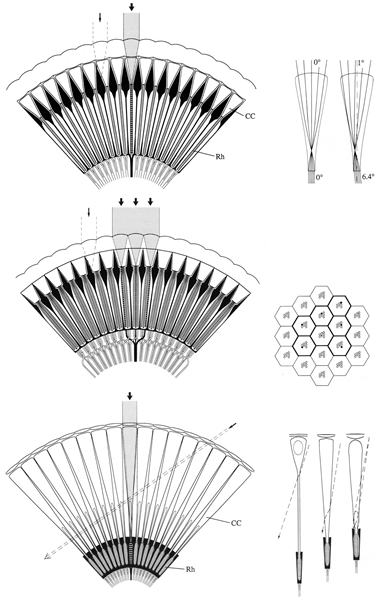
\includegraphics[width=3.0in]{./img/renrituzougan.jpg}
  \caption{連立像眼のしくみ}
  \label{FRenritsu}
\end{figure}

%% \begin{figure}[hn]
%%   \centering
%%   
\includegraphics[width=3.0in]{./img/TEMP}
%%   \caption{連立像眼の例}
%%   \label{FExpparts}
%% \end{figure}

\subsection{重複像眼}

連立像眼が昼行性の種に多く見られるのに対して、重複像眼はガなどの夜行性の種に多く見られる。
重複像眼の特徴としては、色素細胞の色素粒子が光の明暗によって上下に移動する点が挙げられる。
重複像眼の色素細胞は暗いところでは円錐晶体を取り囲むように上部へ移動する。
夜行性の昆虫などの眼が真っ黒に見えることと関連があると考えられる。

\begin{figure}[hn]
  \centering
  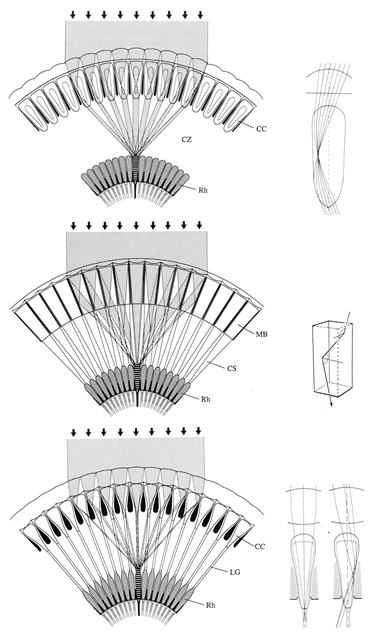
\includegraphics[width=3.0in]{./img/tyoufukuzougan.jpg}
  \caption{重複像眼のしくみ}
  \label{FTyoufuku}
\end{figure}

%% \begin{figure}[hn]
%%   \centering
%%   
\includegraphics[width=3.0in]{./img/TEMP}
%%   \caption{重複像眼の例}
%%   \label{F}
%% \end{figure}

\section{個眼のしくみ}

一般に、複眼が多数の小さな個眼の集合体であり、半球状のドームを形成していることはよく知られている。
個眼の表面は凸レンズ構造をしており、それぞれの形状は六角形もしくは正方形である\figref{}。
個眼のひとつひとつは主にレンズ、色素細胞、円錐晶体そして感桿などから構成されており、複眼の偽瞳孔に関係が深く、外部的な見た目に影響する部位はレンズおよび色素細胞である。

%% \begin{figure}[hn]
%%   \centering
%%   
\includegraphics[width=3.0in]{./img/TEMP}
%%   \caption{個眼の模式図}
%%   \label{F}
%% \end{figure}

%% \begin{figure}[hn]
%%   \centering
%%   
\includegraphics[width=3.0in]{./img/TEMP}
%%   \caption{複眼表面の拡大図}
%%   \label{F}
%% \end{figure}

\section{偽瞳孔}
\label{SPseudopupil}

\secref{SObjective}で述べた偽瞳孔についてより詳細な説明を行う。
偽瞳孔は複眼表面に見られる暗い斑点状の模様であり、チョウやトンボ、セミなどさまざまな昆虫で顕著に現れる。
また、昆虫だけではなくエビやカニなどの複眼を持つ甲殻類にも見られる。

%% \begin{figure}[hn]
%%   \centering
%%   
\includegraphics[width=3.0in]{./img/TEMP}
%%   \caption{昆虫に見られる偽瞳孔}
%%   \label{F}
%% \end{figure}

%偽瞳孔の性質や観察による模様の違いなどを扱った研究は散見されるものの、幾何学的な構造と現れる模様とを関連付けて論じた研究は少ない。
初めに偽瞳孔の現象を発見したのはLeydig\cite{}であり、Leydigは{\it Limulus}の複眼において瞳孔のような暗い斑点を観測し、脊椎動物の瞳孔とは違って外部から観察する方向によって斑点の位置が変化することに言及している。

基本的には、偽瞳孔は中心に位置する暗点とそれを取り囲む6つの暗点から構成されている。
周囲にある6つの暗点は中心の暗点を取り囲む六角形の頂点の位置に見られる。
八木\cite{}は、これらの点のうち中心に位置する暗点をcentral pupil、周囲の位置にある6つの暗点をside pupilと呼称している。
また、side pupilの外側を取り囲むように配置される暗点も存在し、ひとつめのside pupilを中心として先述と同様に六角形状に位置する。
これらの暗点のうち、central pupilとside pupilをのぞいたものはsecond side pupilと呼称されている。
本研究でもこれらの呼称をそのまま用いることにする。

\subsection{Central Pupil}
\label{SSCentralPupil}

八木は色素細胞の位置によってcentral pupilの形状の変化が見られることについて記述している。
色素細胞が円錐晶体の下端にある場合\figref{}、central pupilは比較的丸い形状の単純な暗点として現れる。
この場合、色素細胞が少し円錐晶体の上部へ移動した場合と比較すると大きさはやや小さい。
色素細胞が少しだけ上部へ移動した場合には、偽瞳孔は少し大きくなり暗さを増す。
また、色素細胞がさらに移動し、レンズの近くまで上がってきた場合には、偽瞳孔の形状が六角形に近づいていくという。

全ての偽瞳孔に当てはまるわけではないが、central pupilの中央には茶色もしくは赤みがかった明るい点を示すものがある。
これは、感桿を通して基底膜から反射した光によるものである。
しかしながら、この明点は一部の種をのぞいた他の種ではほとんど見られない。
なぜなら、色素細胞が基底部で円錐晶体を囲っており基底膜への光の進入を抑えているからである。
重複像眼では基底膜および気管のタペータム(tapetum:輝板)からの反射が合わさって赤もしくは琥珀色の明るい輝きになる。

\subsection{Side Pupil}
\label{SSSidePupil}

Side pupilはcentral pupilから同距離に位置し、色素細胞からの間接反射によって起こる。
Central pupilは光が入射したレンズが属している個眼の色素細胞の色を反射しているが、side pupilは光が入射したレンズが属している個眼に隣接する個眼の色素細胞からの反射によって生じる\cite{}。

光が\figref{FSidepupilexplanation}のAのような道筋を通る場合、この個眼の表面はcentral pupilの一部として観測される。
一方、光が\figref{FSidepupilexplanation}のCのような道筋を通る場合、この個眼の表面はside pupilの一部として観測される。
円錐晶体には色素細胞に覆われている部分と覆われていない部分がある。
\figref{FSidepupilexplanation}のBおよびDの道筋を通る視線は、色素細胞に覆われていない円錐晶体の一部に到達している。
通常、これらの位置にぶつかった光は円錐晶体の奥にある体液の色を反射し薄い色として観測される。

角度を変えながらひとつの個眼のレンズを観測すると、ある特定の角度の範囲内で円錐晶体の壁面に沿った色素細胞の色を反射することは明らかである。
逆に、円錐晶体において色素細胞のない壁面の色を反射する角度の範囲も存在すると言える。
すなわち、複眼表面においてcentral pupilとside pupilの間には色素のない領域が存在することは想像に難くない。
また、second side pupilの生じる原理も同様である。

\begin{figure}[htn]
  \centering
  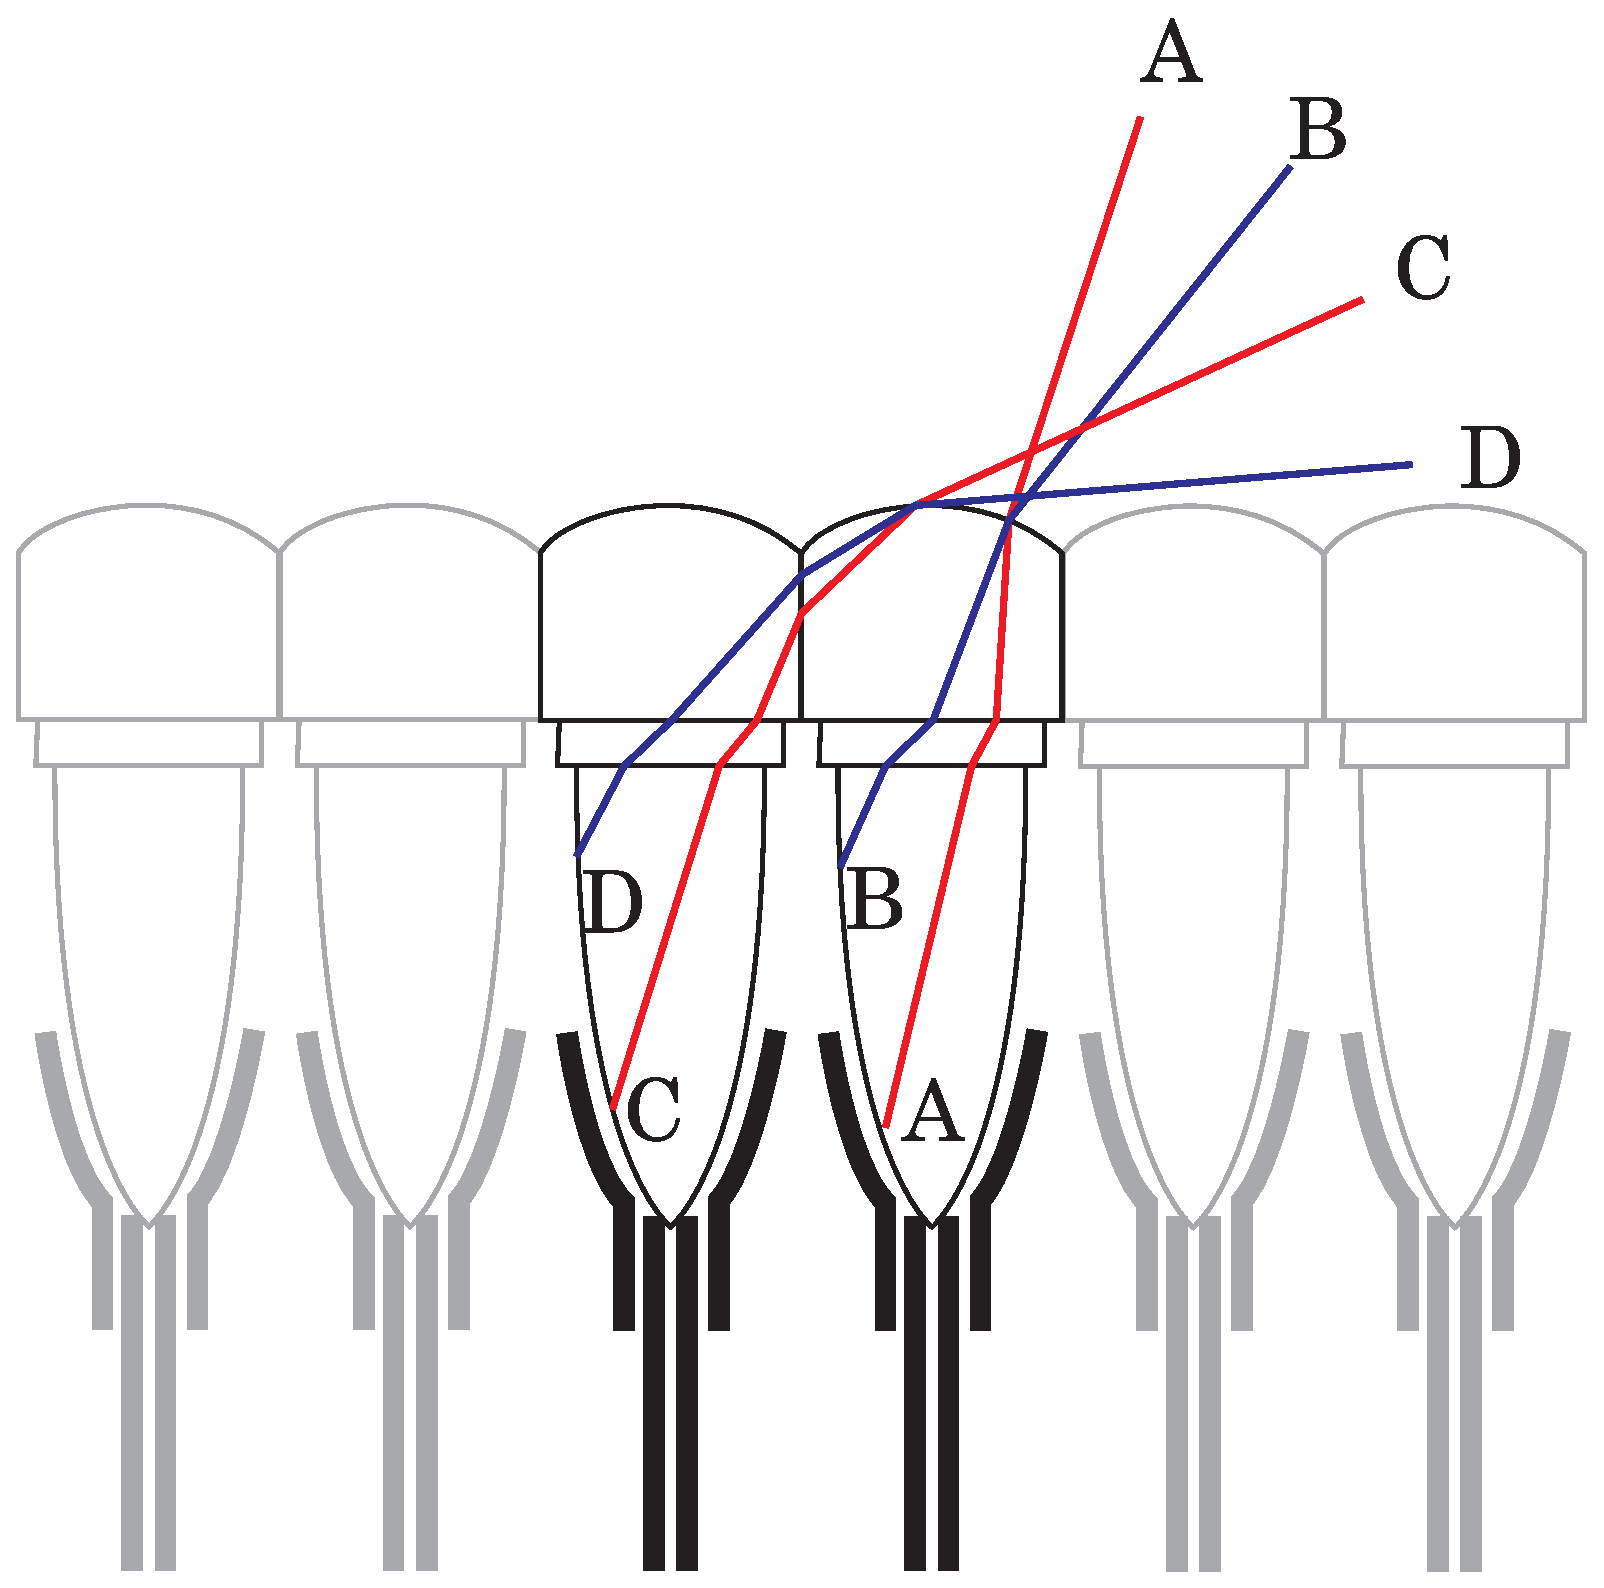
\includegraphics[width=3.5in]{./img/sidepupil_exp}
  \caption{Side pupilの原理}
  \label{FSidepupilexplanation}
\end{figure}

偽瞳孔の暗点はcentral pupil, side pupil, second side pupilの順に色が薄く見えるものも存在する。
その理由としては、side pupilおよびsecond side pupilは隣接する個眼を通過して色素細胞の色を反射するため、通過する個眼のレンズや体液が厚くなり、光が減衰するからであると推測される。

		%3章 周辺知識
\chapter{予備実験}
\label{CExperiment}

\section{実験の目的}
\label{SExperimentPurpose}


実際の複眼の構造や形状は複雑であり、コンピュータグラフィックスにおいて実物の形状を作成したり、実物の構造計算に用いることは難しい。
そこで、複眼の性質を表現するために代替となる形状や近似モデルが必要となる。
本研究では、永田\cite{}が行った偽瞳孔の再現実験をもとにビー玉とパンチングメタルを用いて予備実験を行った。

本実験における第一の目的は、 偽瞳孔の発生原理を理解し、物理現象に落としこむことである。
複眼を扱った関連研究のうち、偽瞳孔の性質や現象について生物学上の考察や解説を行うものは存在するものの、幾何学的なしくみについて言及したものは少ない。
そのため、実物を観察することによって物理現象としてのしくみを明らかにし、開発の足がかりとする必要があった。
第二の目的は、実装を行う前に近似手法による偽瞳孔の再現度を確認することである。
永田の実験は複眼の形状を大きく変え、平板と球体として近似している。そのため、コンピュータグラフィックスとして表現するにあたり、適切な手法であることを確認することが望ましい。
そして第三の目的は、レンズや色素細胞に相当するパンチングメタルの穴などの大きさや周期の違いが模様に与える変化を観察することである。

\section{実験方法}
\label{SExperimentMethod}



\section{結果と議論}
\label{SExperimentResult}

		%4章 予備実験
%\chapter{本手法の基礎技術\\ \textcolor{red}{ たぶんこの章は消去する}}
\label{CBasicmethod}



\section{グラフィックスパイプライン}
\label{SGraphicspipeline}

\section{オブジェクトファイルフォーマット}
\label{SObjfileformat}

モデリングソフト等により前もってオブジェクトファイルを作成し、アプリケーションで読み込みを行う。
さらに、物体形状および法線やテクスチャ座標などの情報を元にアプリケーション内でシェーダへの転送データを生成する。
本手法で必要になるオブジェクトファイルのデータは以下の要素である。

\begin{itemize}
\item 頂点座標値
\item 頂点法線ベクトル
\item テクスチャ座標値
\item 面情報
\end{itemize}

頂点座標値および頂点法線ベクトルはそれぞれ3次元の浮動小数点型、テクスチャ座標値は2次元の浮動小数点型の値となっている。
面情報は、頂点座標値、頂点法線ベクトル、テクスチャ座標値のインデックス番号の組み合わせとなっており、面が表す多角形の頂点の数だけこれらの情報が与えられている。
本手法では三角形ポリゴンのみを対象としているため、この組み合わせが3つずつ続く。

\section{GPU処理}
\label{SGpumethod}

\subsection{シェーダ}
\label{SSShader}
画像処理用演算プロセッサ(GPU:Graphics Processing Unit)で処理を行うのはシェーダとよばれるプログラムであり、このシェーダよって演算処理が実行される。
シェーダ(shader)ではライティング(光源計算)、シェーディング(陰影処理)およびレンダリング(画像ピクセル化)を行う。
本手法では、リアルタイム処理を行うため、プログラマブルパイプライン
     %5章 本手法の基礎技術
\chapter{提案手法}
\label{CMethod}

\secref{SObjective}で述べたように、本研究の目的は複眼表面に観測される光学的現象をリアルタイムレンダリングによって表現することである。
本章では、レンダリング時の計算アルゴリズムについて詳細に解説していく。
まず、\secref{SFramework}で本手法で用いた複眼の近似モデルを提案する。
次に\secref{SObjfile}では、アプリケーションから画像処理用演算プロセッサ(GPU)へと転送するデータと、その生成時に用いた計算アルゴリズムを説明する。
そして\secref{SGpumethod}では、画像処理用演算プロセッサにおいて描画色を求める手法を説明する。

\section{フレームワーク}
\label{SFramework}

\subsection{複眼モデル}
\label{SSModel}

\begin{figure}[h]
  \centering
  
\includegraphics[width=3.0in]{./img/TEMP}
  \caption{シェーディングモデル}{\begin{itemize}\item ポリゴンの直下にレンズとして球体を配置。\item 距離を開けてポリゴンと平行にテクスチャ平面を配置。\end{itemize}}
  \label{FModel}
\end{figure}

\chapref{CExperiment}で取り上げた実験をもとに、シェーダアルゴリズムに図のようなモデルを採択した\figref{FModel}。
ポリゴン直下に屈折レンズの役割を果たす球体を配置し、表面を埋め尽くすように多数配置している。
さらに、テクスチャ平面と称してポリゴンと平行な位置にテクスチャ情報を取得するための平面を配置している。
テクスチャ平面は、\secref{}で説明した色素細胞の役割を担っている。
レンズによって屈折された光はテクスチャ平面へ到達し、テクスチャ平面上の情報から色への影響を決定する。

続いて、モデルの利点を説明する。
まず、このモデルは複雑な複眼の構造を球や平面などの単純な幾何立体の集合として扱うことができる。そのため、光の屈折等を計算する際に、きわめて軽量な計算量で済むという利点がある。
次に、\chapref{CExperiment}の実験は永田\cite{}が示しているように偽瞳孔現象の特徴を十分に再現している。
ゆえに、近似モデルとして十分に目的を果たすことが期待できる。


\subsection{アルゴリズムの全体像}
\label{SSAlgorithm}

\begin{figure}[h]
  \centering
  
\includegraphics[width=3.0in]{./img/TEMP}
  \caption{アルゴリズムフレームワーク}
  \label{FAlgoframework}
\end{figure}

本手法のアルゴリズムの全体像を説明する。
本手法の構成は大きく分けると、最初に複眼表面を適用する形状データの作成、次にアプリケーションにおいて計算に用いるデータの処理。
そして最後に偽瞳孔による光の減衰量計算および光源、陰影処理等がなされる\figref{FAlgoframework}。
アプリケーションでは通常の手法で作成されたオブジェクトファイル情報を加工し、計算に必要な変数をGPU(シェーダ)へ送る。
シェーダでは屈折などを考慮した物理計算を行い、最終的に画面に描画する色情報を計算する。

\section{計算用データ}
\label{SObjfile}

読み込んだオブジェクトファイルデータから計算用のベクトルデータを生成する。
この処理はアプリケーション内で一度だけ行われ、プログラマブルシェーダへ転送されたのち保持される。


頂点情報としてにシェーダへ転送されるデータは、頂点座標値、頂点法線ベクトル、テクスチャ座標値、そして後述する接ベクトル情報である。
これらのうち頂点座標値および頂点法線ベクトルは更新されず、オブジェクトファイルから読み取った値を面情報にしたがって順次バーテックスバッファオブジェクトの形で配列情報として転送される。
テクスチャ座標値はユーザ指定の浮動小数点型の値であるテクスチャ解像度$R_t$を以下のように乗算し転送される。

\begin{equation}
{\bm T_{vert}} = R_{t}{\bm T_{obj}}
\end{equation}

\noindent
ここで、$\bm{T}_{obj}$は作成した形状データから読み込んだテクスチャ座標値、$\bm{T}_{vert}$は頂点シェーダ(\secref{SSShader})へ転送されるテクスチャ座標値である。

本手法ではテクスチャ座標値をもとに屈折レンズ(\secref{SSModel})の配置を決定しているため、$R_t$を変更することで複眼表面のレンズの配置すなわち表面構造の細かさを任意に変更することができる。

これらの頂点情報の他にシェーダへ与えられる定数などの情報はプログラマブルシェーダ内の変数として適宜転送される。

\subsection{テクスチャ座標軸方向3次元単位ベクトル}
\label{SSUnitvec}

通常、2次元空間上のデータであるテクスチャは、テクスチャ座標値と空間上の点との対応づけにより3次元空間上に描写される。
すなわち、3次元空間における面は2次元の座標空間として考えることができる\figref{}。
そこで、3次元空間内の情報から2次元情報であるテクスチャ座標値を算出するためには、異なる次元同士を橋渡しする変数が必要になる。

本手法では、オブジェクト上の各位置におけるテクスチャ座標系の単位ベクトルを3次元ベクトルとして表すことによって、異なる次元の情報を結びつけている。
本項では、2次元ベクトルであるテクスチャ座標空間の単位ベクトルを、3次元空間上の3次元ベクトルとして表す方法について述べる。
また、3次元空間上のテクスチャ座標軸方向単位ベクトルを用いると、ポリゴン上の任意の点においてテクスチャ座標値を逆算できるようになる。

ポリゴン上のある位置におけるテクスチャ座標空間の軸方向の単位ベクトルを3次元ベクトル$\bm{U}_p, \bm{V}_p$として表すと、ポリゴン上の任意点$\bm{P}$は$\bm{U}_p, \bm{V}_p$を利用して以下のように表現することができる。

\begin{equation}
\bm{P} = \bm{P}_c + a\bm{U}_p + b\bm{V}_p
\label{EPuv}
\end{equation}

\noindent
ここで、$\bm{P}_c$は既知の点$\bm{P}_e$およびそのテクスチャ座標値$(a_e, b_e)$によって

\begin{equation}
\bm{P}_c = \bm{P}_e - a_e\bm{U}_p - b_e\bm{V}_p
\label{EPc}
\end{equation}

\noindent
\equref{EPc}のように表される。また、\equref{EPuv}の$a$および$b$は点$\bm{P}$におけるテクスチャ座標値$(a, b)$を表している。
すなわち、3次元空間上のテクスチャ座標軸方向単位ベクトル$\bm{U}_p, \bm{V}_p$が既知であれば、\equref{EPuv}の係数を利用してポリゴン上の任意の点におけるそのテクスチャ座標値$(a, b)$を逆算することが可能になる。
本手法では、シェーダでの処理に3次元ベクトル$\bm{P}_c$, $\bm{U}_p$および$\bm{V}_p$が必要となるため、これらの値を作成しシェーダへ転送する必要がある。

テクスチャ座標軸方向3次元単位ベクトル$\bm{U}_p$および$\bm{V}_p$は以下の手順で求める。
$\bm{U}_p$および$\bm{V}_p$はポリゴン毎に変化するベクトル変数であり、ポリゴンを構成する各頂点の頂点情報としてバッファに格納される。
まず、本手法で対象としている三角形ポリゴンの各頂点の頂点座標値を$\bm{P}_0,\bm{P}_1,\bm{P}_2$とし、テクスチャ座標値を$\bm{T}_0,\bm{T}_1,\bm{T}_2$とする。
ここでは、頂点座標値が3次元ベクトルであるのに対してテクスチャ座標値が2次元ベクトルであることに留意し、ポリゴン上で両者の対応関係を明確にしていく。

三角形ポリゴンは3次元空間上における平面を一意に表すことができるため、この平面に対応するベクトルを$\bm{P}_0,\bm{P}_1,\bm{P}_2$および$\bm{T}_0,\bm{T}_1,\bm{T}_2$から求めていく。

\begin{figure}[h]
  \centering
  
\includegraphics[width=3.0in]{./img/TEMP}
  \caption{ポリゴン上における頂点座標値およびテクスチャ座標値の関係}
  \label{FVertexandtexture}
\end{figure}


頂点座標値から相対ベクトル$\bm{P}_{10}$,$\bm{P}_{20}$を以下のように定義する。

\begin{equation}
\bm{P}_{10} = \bm{P}_1 - \bm{P}_0
\label{EP10}
\end{equation}

\begin{equation}
\bm{P}_{20} = \bm{P}_2 - \bm{P}_0
\label{EP20}
\end{equation}


同様に、テクスチャ座標値から相対ベクトル$\bm{T}_{10}$,$\bm{T}_{20}$を以下のように定義する。

\begin{equation}
\bm{T}_{10} = \bm{T}_1 - \bm{T}_0
\label{ET10}
\end{equation}

\begin{equation}
\bm{T}_{20} = \bm{T}_2 - \bm{T}_0
\label{ET20}
\end{equation}

これらの相対ベクトルはポリゴンのエッジに相当し、それぞれ平面上の変位を表すベクトルとなっている\figref{FVertexandtexture}。

さて、テクスチャ座標軸方向3次元単位ベクトル$\bm{U}_p$および$\bm{V}_p$は$i,j,k,l$を適当な係数として以下のように表すことができる。

\begin{equation}
\bm{U}_p = i\bm{P}_{10} + j\bm{P}_{20}
\label{EUp}
\end{equation}

\begin{equation}
\bm{V}_p = k\bm{P}_{10} + l\bm{P}_{20}
\label{EVp}
\end{equation}

そして、係数$i,j,k,l$は$\bm{T}_{10}$および$\bm{T}_{20}$から導くことができる。


\begin{figure}[h]
  \centering
  
\includegraphics[width=3.0in]{./img/TEMP}
  \caption{平面上の変位ベクトル}
  \label{FAtoB}
\end{figure}

続いて、ポリゴン平面上の任意の位置にある点$A$および$B$を考える\figref{FAtoB}。
点$A$の頂点座標値を$\bm{P}_A$そして点$B$の頂点座標値を$\bm{P}_B$とすると、点$A$および点$B$の3次元空間上における位置の変位は、$c,d$を適当な係数として以下のように表すことができる。

\begin{eqnarray}
\bm{P}_{AB} &=& \bm{P}_A - \bm{P}_B\nonumber\\
           &=& c\bm{P}_{10} +  d\bm{P}_{20}  
\label{EPab}
\end{eqnarray}

さらに、$\bm{P}_{10}$と$\bm{T}_{10}$および、$\bm{P}_{20}$と$\bm{T}_{20}$がポリゴン上で対応関係にあることから、点$A$のテクスチャ座標値を$\bm{T}_A$そして点$B$のテクスチャ座標値を$\bm{T}_B$とすると以下の式が成り立つ。

\begin{eqnarray}
\bm{T}_{AB} &=& \bm{T}_A - \bm{T}_B\nonumber\\
           &=& c\bm{T}_{10} +  d\bm{T}_{20}  
\label{ETab}
\end{eqnarray}

ここで、$i,j,k,l$を用いて

\begin{equation}
i\bm{T}_{10} + j\bm{T}_{20} = 
\begin{pmatrix}
1\\
0
\end{pmatrix}
\label{EUnit2u}
\end{equation}

\begin{equation}
k\bm{T}_{10} + l\bm{T}_{20} = 
\begin{pmatrix}
0\\
1
\end{pmatrix}
\label{EUnit2v}
\end{equation}

\noindent
とし、テクスチャ座標空間をUV座標で表すと、2次元空間内において\equref{EUnit2u}はU軸単位ベクトル、\equref{EUnit2v}はV軸単位ベクトルを表すことになる。
さらに、\equref{EPab}および\equref{ETab}の対応関係から\equref{EUp}および\equref{EVp}を導くことができる。

2次正方行列$\bm{A} = (\bm{T}_{10}, \bm{T}_{20})$とすると\equref{EUnit2u}と\equref{EUnit2v}から

\begin{equation}
\bm{A} 
\begin{pmatrix}
i &k\\
j &l
\end{pmatrix}
=
\begin{pmatrix}
1 &0\\
0 &1
\end{pmatrix}
\label{EAx=I}
\end{equation}

\noindent
\equref{EAx=I}が成り立ち、これを変形すると以下のようになる。

\begin{eqnarray}
\begin{pmatrix}
i &k\\
j &l
\end{pmatrix}
&=& \bm{A}^{-1}
\begin{pmatrix}
1 &0\\
0 &1
\end{pmatrix}\nonumber\\
&=& \bm{A}^{-1}
\label{EIjkl}
\end{eqnarray}

\noindent
以上から$i,j,k,l$を求めることができた。

さらに、\equref{EPc}において$\bm{P}_e = \bm{P}_0$, $(a_e, b_e) = \bm{T}_0$として$\bm{P}_c$を作成し、$\bm{U}_p$, $\bm{V}_p$と合わせて利用する。


			%6章 提案手法
\chapter{結果と考察}
\label{CResult}

%% \textcolor{red}{****メモ始め****}
%% \begin{itemize}
%% \item 使用したテクスチャとかの画像を載せる
%% \item 形状モデルのワイヤフレーム画像
%% \item ポリゴン数とか面の数、頂点の数でテーブルを作成する
%% \item 球がひとつの場合の実物との比較
%% \item 平面オブジェクトに対する実行結果と解像度$R_t$の評価
%% \item 球体オブジェクト
%% \item 実行結果の処理速度のグラフを作る
%% \item 結果の実物との比較
%% \item 定性的評価
%% \item さまざまなオブジェクトへの適用
%% \item 鹿児島アートフェスタ
%% \end{itemize}
%% \textcolor{red}{****メモ終わり****}

\section{実装方法および実行環境}
\label{SEnvironment}

本手法ではグラフィックスライブラリとしてOpenGL(オープンジーエル: Open Graphics Library)を利用し、プログラムの実装にあたってはC++言語を用いている。
本手法を適用する形状データはAutodesk Maya \textcolor{red}{2013}で作成したオブジェクトファイルを使って作成した。

プログラムの実行に使用した計算機のハードウェア構成は\tabref{tab:experiment-hadrware}のとおりである。

\begin{table}
\centering
\caption{実行環境 \label{tab:experiment-hadrware}}
\begin{tabular}{r|l}
\hline
CPU & Intel Core i7 960 3.20 GHz \\ \hline
メモリ & 30 GB \\ \hline
GPU & NVIDIA GeForce GTX 660 \\ \hline
%グラフィックメモリ & 3 GB GDDR5 \\ \hline
\end{tabular}
\end{table}

%------------------------------------------------------------------------------------------
\section{処理系}
\label{S}

\subsection{内処理、外処理}
\label{SSInnerOuterProcess}

\chapref{CMethod}で述べた隣接球を通過する光の挙動について、平面オブジェクトおよび球体オブジェクトを例に問題点を指摘する。
%% 本手法で用いた複眼の近似モデル(\secref{SSModel})では、個眼のレンズの代わりに球体レンズを利用している。
%% また、本来は予備実験\secref{SSMarbleOnHole}のように最密に球を配置することが理想であるが、本手法では評価実験のためにアルゴリズムが簡略な格子状の配置を採択している。**methodに追記する**
本手法では、球体レンズ同士の間にできる隙間を埋めるために、球の直径を球同士の中心距離よりも大きく設定している(\secref{SSMultiRefraction})。
また、複数の球を通過する光を想定し、光が球の外部を経由して隣接する球に入射する場合のアルゴリズムを実装していた。
しかし、外部を経由する場合の実装(以下、外部通過処理)によって得られる結果画像にはノイズが多く、求める画像とは異なる結果となってしまった\figref{FNoise}。
\begin{figure}[htbp]
  \centering
\subfigure[平面オブジェクト]{
\includegraphics*[width=.45\columnwidth]{./img/screenshot/sphere/Noise/pscreenshot005.bmp}
\label{FNoisePlane}}
\subfigure[球体オブジェクト]{
\includegraphics*[width=.45\columnwidth]{./img/screenshot/sphere/Noise/screenshot000.bmp}
\label{FNoiseSphere}}
  \caption{外部通過処理に見られるノイズ}
  \label{FNoise}
\end{figure}
そのため、手法の修正として外部通過処理を実装から排除し、球の内部から内部への光の通過を考慮した実装(以下、内部通過処理)のみを採択することにした。

外部通過処理を排除しても、本手法で想定される範囲内では問題はないと考えられる。
理由として、外部通過処理と内部通過処理のそれぞれによって得られる画像にはノイズの有無以外に大きな差異が観測されなかったことと、球の半径を十分に大きい値で設定すれば、球の外部を経由して隣接する球に入射する光はあまり存在しないと推測されることが挙げられる。
ゆえに、本章での考察は主に内部通過処理によって得られるものに対して行う。

%------------------------------------------------------------------------------------------

\section{ジオメトリ}
\label{S}

\subsection{レンズ半径と偽瞳孔の数}
\label{SS}

本手法では、レンズの位置座標とレンズの半径は独立して扱うことができる。
\secref{SSInnerOuterProcess}でも述べたように、本手法では配置された球体レンズ同士の間の隙間を埋めるため、球の半径を球同士が接するよりも大きい値で設定しており、球の半径によって光の入射する領域のレンズの曲率が変化する。
すなわち、球の半径$r$の設定値によって複眼の外観が変化するため、両者の関係について考察を行う。
以下ではテクスチャに\figref{}を使用しており、テクスチャ解像度$R_t = 300$を使用している。

\begin{figure}[htbp]
  \centering
\subfigure[$r = 0.03$]{
\includegraphics*[width=.3\columnwidth]{./img/screenshot/sphere/Radius/1_30/screenshot000.bmp}
\label{FRadius003-0}}
\subfigure[$r = 0.03$]{
\includegraphics*[width=.3\columnwidth]{./img/screenshot/sphere/Radius/1_30/screenshot001.bmp}
\label{FRadius003-1}}
\subfigure[$r = 0.03$]{
\includegraphics*[width=.3\columnwidth]{./img/screenshot/sphere/Radius/1_30/screenshot002.bmp}
\label{FRadius003-2}}\\
\subfigure[$r = 0.04$]{
\includegraphics*[width=.3\columnwidth]{./img/screenshot/sphere/Radius/1_24/screenshot000.bmp}
\label{FRadius004-0}}
\subfigure[$r = 0.04$]{
\includegraphics*[width=.3\columnwidth]{./img/screenshot/sphere/Radius/1_24/screenshot001.bmp}
\label{FRadius004-1}}
\subfigure[$r = 0.04$]{
\includegraphics*[width=.3\columnwidth]{./img/screenshot/sphere/Radius/1_24/screenshot002.bmp}
\label{FRadius004-2}}\\
\subfigure[$r = 0.06$]{
\includegraphics*[width=.3\columnwidth]{./img/screenshot/sphere/Radius/1_16/screenshot000.bmp}
\label{FRadius006-0}}
\subfigure[$r = 0.06$]{
\includegraphics*[width=.3\columnwidth]{./img/screenshot/sphere/Radius/1_16/screenshot001.bmp}
\label{FRadius006-1}}
\subfigure[$r = 0.06$]{
\includegraphics*[width=.3\columnwidth]{./img/screenshot/sphere/Radius/1_16/screenshot002.bmp}
\label{FRadius006-2}}\\
\subfigure[$r = 0.10$]{
\includegraphics*[width=.3\columnwidth]{./img/screenshot/sphere/Radius/1_10/screenshot000.bmp}
\label{FRadius010-0}}
\subfigure[$r = 0.10$]{
\includegraphics*[width=.3\columnwidth]{./img/screenshot/sphere/Radius/1_10/screenshot001.bmp}
\label{FRadius010-1}}
\subfigure[$r = 0.10$]{
\includegraphics*[width=.3\columnwidth]{./img/screenshot/sphere/Radius/1_10/screenshot002.bmp}
\label{FRadius010-2}}
  \caption{レンズ半径$r$と偽瞳孔の数の関係}
  \label{FRadiusAndNumber}
\end{figure}

比較画像\figref{FRadiusAndNumber}からレンズ半径が大きくなるにつれて観測される偽瞳孔の数は増加していることがわかる。
これは、半径が小さく曲率が大きければ個眼の端でのレンズ表面への進入角が小さくなるので、より内側への屈折が起こり、逆に半径が大きく曲率が小さければ、進入角が相対的に大きくなるので屈折の度合いが抑えられ、結果的に隣接する色素細胞テクスチャへ到達する頻度が高くなるためであると考えられる。

再現性を高めるためには、対象生物の個眼のレンズの曲率を測定するか、ユーザが任意の半径値$r$を設定することが必要となるが、ある程度恣意的に結果を操作できる点はユーザビリティにつながるのではないだろうか。
事実、生物種によって観察される偽瞳孔の密度や分布は異なるため、求める結果を得るための試行錯誤が必要である。

\subsection{視点との距離による偽瞳孔の分布}
\label{SSViewDist}

\secref{SSMarbleOnHole}では、偽瞳孔に相当する黒点の装置に対する大きさは視点との距離によって変化した。
%%%%%%%%%%%%%%%%%%%%%%%%%%

\subsection{歪みとテクスチャの関係}
\label{SSDistortion}

結果画像の一部には歪みが生じている部分が存在する\figref{FTexTortion}。
これは、オブジェクトに適用されたテクスチャに継ぎ目が存在し、なめらかに接続していないことが原因である。
本手法の特性上、曲面オブジェクトの表面に対しては格子状にテクスチャを適用する必要があるため、立体表面でテクスチャの歪みが生じることは避けられない。
すなわち、閉じた立体ではなく開いた曲面もしくはテクスチャの継ぎ目を表示しないモデルを使用するなどの工夫が要求される。
また、この問題はレンズ球の配置条件によって生じるので、レンズ球の配置アルゴリズムを改善するなどの対応策が今後求められる。

\begin{figure}[htbp]
  \centering
\subfigure[テクスチャマップ]{
\includegraphics*[width=.45\columnwidth]{./img/screenshot/sphere/Distortion/tex_tortion1.png}
\label{FTexTortion1}}
\subfigure[結果]{
\includegraphics*[width=.45\columnwidth]{./img/screenshot/sphere/Distortion/screenshot000.bmp}
\label{FTexTortion1-s}}\\
\subfigure[テクスチャマップ]{
\includegraphics*[width=.45\columnwidth]{./img/screenshot/sphere/Distortion/tex_tortion2.png}
\label{FTexTortion2}}
\subfigure[結果]{
\includegraphics*[width=.45\columnwidth]{./img/screenshot/sphere/Distortion/screenshot001.bmp}
\label{FTexTortion2-s}}\\
\subfigure[テクスチャマップ]{
\includegraphics*[width=.45\columnwidth]{./img/screenshot/sphere/Distortion/tex_tortion3.png}
\label{FTexTortion3}}
\subfigure[結果]{
\includegraphics*[width=.45\columnwidth]{./img/screenshot/sphere/Distortion/screenshot002.bmp}
\label{FTexTortion3-s}}\\
  \caption{テクスチャの継ぎ目}
  \label{FTexTortion}
\end{figure}

\newpage
\subsection{さまざまなテクスチャ}
\label{SS}

本手法ではテクスチャを変更することにより外観が大幅に変化する。
基本的には、モデルであるパンチングメタルを模して黒点のテクスチャをタイリングする。
以下に、本手法で用いた基本のテクスチャおよび任意のテクスチャを使用した場合の結果を紹介する\figref{FBaseTextureAndResult}。

\begin{figure}[htbp]
  \centering
\subfigure[基本テクスチャ]{
\includegraphics*[width=.45\columnwidth]{./img/screenshot/texture/spot.jpg}
\label{FBaseTexture}}\\
\subfigure[結果画像]{
\includegraphics*[width=.45\columnwidth]{./img/screenshot/texture/spot.bmp}
\label{FBaseResult}}
  \caption{基本テクスチャと適用結果}
  \label{FBaseTextureAndResult}
\end{figure}

\begin{figure}[htbp]
  \centering
\subfigure[テクスチャ]{
\includegraphics*[width=.3\columnwidth]{./img/screenshot/texture/a.jpg}
\label{FTex1}}
\subfigure[結果]{
\includegraphics*[width=.45\columnwidth]{./img/screenshot/texture/a.bmp}
\label{FTexResult1}}\\
\subfigure[テクスチャ]{
\includegraphics*[width=.3\columnwidth]{./img/screenshot/texture/colormap.jpg}
\label{FTex2}}
\subfigure[結果]{
\includegraphics*[width=.45\columnwidth]{./img/screenshot/texture/colormap.bmp}
\label{FTexResult2}}\\
\subfigure[テクスチャ]{
\includegraphics*[width=.3\columnwidth]{./img/screenshot/texture/spot5.jpg}
\label{FTex3}}
\subfigure[結果]{
\includegraphics*[width=.45\columnwidth]{./img/screenshot/texture/spot5.bmp}
\label{FTexResult3}}\\
  \caption{テクスチャの変更による外観の変化}
  \label{FTexResults}
\end{figure}

%------------------------------------------------------------------------------------------
\newpage
\section{パラメータと実行速度}
\label{SParameterAndExeTime}

それぞれのパラメータに応じて得られる結果画像や実行速度について比較、検討を行う。
評価を行うパラメータは光が通過する球の数の上限値、カメラとの距離、テクスチャの解像度である。
対象オブジェクトは以下に示す平面オブジェクトおよび球体オブジェクトとする。
\begin{figure}[htbp]
  \centering
\subfigure[平面オブジェクト(ワイヤフレーム)]{
\includegraphics*[width=.45\columnwidth]{./img/screenshot/plane_wireframe.png}
\label{FNoisePlane}}
\subfigure[球体オブジェクト(ワイヤフレーム)]{
\includegraphics*[width=.45\columnwidth]{./img/screenshot/sphere_wireframe.png}
\label{FNoiseSphere}}
  \caption{評価オブジェクト(ワイヤフレーム表示)}
  \label{FEvalObject}
\end{figure}

\begin{table}[htbp]
\centering
\caption{オブジェクト情報 \label{TObjectInfo}}
\begin{tabular}{r||l|l|}
\hline
 & 平面オブジェクト & 球体オブジェクト \\ \hline
頂点数 & 4 & 9218 \\ \hline
面の数 & 2 & 18432 \\ \hline
ポリゴンの種類 & 三角形 & 三角形 \\ \hline
%グラフィックメモリ & 3 GB GDDR5 \\ \hline
\end{tabular}
\end{table}

\subsection{隣接球の処理ON/OFF}
\label{SSLimitNeighborSphere}

光がどの程度の回数、隣接球を通過する必要があるのかについての考察を行う。
光が複眼表面に対して平行に近い角度で入射した場合、光はひとつの球だけではなくふたつ以上の球を通過すると考えられる。
通過する球の数が増えればそれだけ処理に時間がかかるため、通過する球の数には上限値を設定する必要がある。
すなわち、物理的な正確さと処理速度はトレードオフの関係にあると言える。

では、通過する球の数の上限値を変化させることによって得られる結果について議論を行う。
上限値を設定することによる操作をここでは隣接球処理と呼ぶことにする。
以下では上限値$l = 0,1,2,3, ......$のように設定し、上限値$l$が$0$の場合には隣接球処理を行わないこととする。
すなわち、$l = 0$の場合、最初の球に入射した光は他のいかなる隣接球にも入射せずテクスチャ平面(\secref{SSModel})へ到達するものとして考える。
以下にまず、各$l$の値に対する結果を示す\figref{FLimitCompare1}\figref{FLimitCompare2}。
テクスチャは\figref{FBaseTexture}を使用しており、球の半径$r$の値は約$3.3 \times 10^{-2}$、テクスチャ解像度$R_t = 300$を使用している。

\begin{figure}[htbp]
  \centering
\subfigure[$l = 0$]{
\includegraphics*[width=.45\columnwidth]{./img/screenshot/sphere/RefracLimit/000/screenshot002.bmp}
\label{FLimit0-4}}
\subfigure[$l = 1$]{
\includegraphics*[width=.45\columnwidth]{./img/screenshot/sphere/RefracLimit/001/screenshot002.bmp}
\label{FLimit1-4}}\\
\subfigure[$l = 2$]{
\includegraphics*[width=.45\columnwidth]{./img/screenshot/sphere/RefracLimit/002/screenshot002.bmp}
\label{FLimit2-4}}
\subfigure[$l = 3$]{
\includegraphics*[width=.45\columnwidth]{./img/screenshot/sphere/RefracLimit/003/screenshot002.bmp}
\label{FLimit3-4}}\\
\subfigure[$l = 5$]{
\includegraphics*[width=.45\columnwidth]{./img/screenshot/sphere/RefracLimit/005/screenshot002.bmp}
\label{FLimit5-4}}
\subfigure[$l = 10$]{
\includegraphics*[width=.45\columnwidth]{./img/screenshot/sphere/RefracLimit/010/screenshot002.bmp}
\label{FLimit10-4}}
  \caption{上限値による画像の変化1}
  \label{FLimitCompare1}
\end{figure}

\begin{figure}[htbp]
  \centering
\subfigure[$l = 0$]{
\includegraphics*[width=.45\columnwidth]{./img/screenshot/sphere/RefracLimit/000/screenshot001.bmp}
\label{FLimit0-3}}
\subfigure[$l = 1$]{
\includegraphics*[width=.45\columnwidth]{./img/screenshot/sphere/RefracLimit/001/screenshot001.bmp}
\label{FLimit1-3}}\\
\subfigure[$l = 2$]{
\includegraphics*[width=.45\columnwidth]{./img/screenshot/sphere/RefracLimit/002/screenshot001.bmp}
\label{FLimit2-3}}
\subfigure[$l = 3$]{
\includegraphics*[width=.45\columnwidth]{./img/screenshot/sphere/RefracLimit/003/screenshot001.bmp}
\label{FLimit3-3}}\\
\subfigure[$l = 5$]{
\includegraphics*[width=.45\columnwidth]{./img/screenshot/sphere/RefracLimit/005/screenshot001.bmp}
\label{FLimit5-3}}
\subfigure[$l = 10$]{
\includegraphics*[width=.45\columnwidth]{./img/screenshot/sphere/RefracLimit/010/screenshot001.bmp}
\label{FLimit10-3}}\\
  \caption{上限値による画像の変化2}
  \label{FLimitCompare2}
\end{figure}



\newpage
結果画像からは$l = 0$の場合とそれ以外とで顕著な差異が見られ、$l = 1$および$l = 2$の場合とそれ以外の場合でわずかな差異が確認できた。
また、$l = 3$以上の場合については肉眼で判別できるほどの差異は見つからなかった。
まず、$l = 0$の場合とそれ以外との差異について述べる。
$l = 0$の場合、side pupil(\secref{SSSidePupil})の存在が確認できるものの、他の場合と比較するとやや黒色が薄く、隣接球処理をした場合のほうがはっきりとしたside pupilとなっていることがわかる。
\begin{figure}[htbp]
  \centering
\subfigure[$l = 1$]{
\includegraphics*[width=.75\columnwidth]{./img/screenshot/sphere/RefracLimit/001/pupil4_explain.png}
\label{FPupil4}}\\
\subfigure[$l = 1$]{
\includegraphics*[width=.75\columnwidth]{./img/screenshot/sphere/RefracLimit/001/pupil3_explain.png}
\label{FPupil3}}
  \caption{各偽瞳孔の名称および場所}
  \label{FPseudopupilName}
\end{figure}
$l = 1,2$の場合とそれ以外の場合を代表して$l = 3$の場合について比較を行うと、球体オブジェクトの縁において有意差が見られる。
$l = 1$の場合、side pupilのさらに外側に位置するsecond side pupil(\figref{FLimitCompare3}\figref{FLimitCompare4}緑部)のあたりは$l = 3$の場合よりも黒点の形状が曖昧となっている。
逆に、$l = 2$の場合は$l = 1,3$の場合と比較して白色領域が広くなっている。
特に、$l = 1$の場合では\figref{FLimitCompare3}\figref{FLimitCompare4}黄部付近のsecond side pupilがやや大きいのに対して、それ以降の場合では縮小していることが顕著に観測される。
以上のことから、偽瞳孔のside pupilおよびsecond side pupilには隣接球を通過する光が影響していることがわかり、\secref{SSSidePupil}の理論と一致する。

続いて、実行速度と$l$の関係を示す\figref{FExetimeAndL}。
\begin{figure}[htbp]
  \centering
\subfigure[平均値]{
\includegraphics*[width=.75\columnwidth]{./img/graph/exetime_average.png}
\label{FExetimeAverage}}\\
\subfigure[実測値]{
\includegraphics*[width=.75\columnwidth]{./img/graph/exetime_samp.png}
\label{FExetimeSamp}}
  \caption{実行速度と$l$の関係}
  \label{FExetimeAndL}
\end{figure}
平均値\figref{FExetimeAverage}と実測値\figref{FExetimeSamp}のいずれのグラフからも、実行速度と通過隣接球上限値$l$は線形の関係であることがわかる。
さらに、リアルタイムの基準が60 fpsであるとすると、今回の球体オブジェクトの場合では$l=900$付近がリアルタイムの限界値であると考えられる。
また、先述のように$l=3$以上では結果画像に有意な差が見られないことから、$l$の設定値は$10^1$オーダーで十分であると言える。

%% \textcolor{red}{実行速度と$l = 10$程度で十分とかそういう話}


\newpage
\begin{figure}[htbp]
  \centering
\subfigure[$l = 0$]{
\includegraphics*[width=.45\columnwidth]{./img/screenshot/sphere/RefracLimit/000/marker4.png}
\label{FMarker0}}
\subfigure[$l = 1$]{
\includegraphics*[width=.45\columnwidth]{./img/screenshot/sphere/RefracLimit/001/marker4.png}
\label{FMarker1}}\\
\subfigure[$l = 2$]{
\includegraphics*[width=.45\columnwidth]{./img/screenshot/sphere/RefracLimit/002/marker4.png}
\label{FMarker2}}
\subfigure[$l = 3$]{
\includegraphics*[width=.45\columnwidth]{./img/screenshot/sphere/RefracLimit/003/marker4.png}
\label{FMarker3}}\\
  \caption{上限値による画像の変化比較3}
  \label{FLimitCompare3}
\end{figure}

\begin{figure}[htbp]
  \centering
\subfigure[$l = 0$]{
\includegraphics*[width=.45\columnwidth]{./img/screenshot/sphere/RefracLimit/000/marker.png}
\label{FMarker0}}
\subfigure[$l = 1$]{
\includegraphics*[width=.45\columnwidth]{./img/screenshot/sphere/RefracLimit/001/marker.png}
\label{FMarker1}}\\
\subfigure[$l = 2$]{
\includegraphics*[width=.45\columnwidth]{./img/screenshot/sphere/RefracLimit/002/marker.png}
\label{FMarker2}}
\subfigure[$l = 3$]{
\includegraphics*[width=.45\columnwidth]{./img/screenshot/sphere/RefracLimit/003/marker.png}
\label{FMarker3}}\\
  \caption{上限値による画像の変化比較4}
  \label{FLimitCompare4}
\end{figure}


\newpage
\subsection{カメラとの距離による実行速度}
\label{SSCameraDist}

\subsection{テクスチャ解像度}
\label{SSTexReso}


%------------------------------------------------------------------------------------------

\section{その他}
\label{S}


\section{さまざまなオブジェクト}
\label{S}

\section{応用事例}
\label{S}





%--前書いてたやつ----------------------------------------------------------------------------------------
%% \newpage
%% \section{平面オブジェクトに適用した結果}
%% \label{SPlaneObject}

%% 本研究で提案した屈折を表現する手法の有用性を評価するため、平面オブジェクトに対して球体レンズを適用する実験を行った。


%% \begin{figure}[htbp]
%%   \centering
%% \subfigure[CAPTIONa]{
%% \includegraphics*[width=.45\columnwidth]{./img/single/screenshot001.bmp}
%% \label{F}}
%% \subfigure[CAPTIONb]{
%% \includegraphics*[width=.45\columnwidth]{./img/single/screenshot002.bmp}
%% \label{F}}\\
%% \subfigure[CAPTIONc]{
%% \includegraphics*[width=.45\columnwidth]{./img/single/screenshot003.bmp}
%% \label{F}}
%% \subfigure[CAPTIONd]{
%% \includegraphics*[width=.45\columnwidth]{./img/single/screenshot004.bmp}
%% \label{F}}\\
%% \subfigure[CAPTIONa]{
%% \includegraphics*[width=.45\columnwidth]{./img/single/screenshot005.bmp}
%% \label{F}}
%% \subfigure[CAPTIONb]{
%% \includegraphics*[width=.45\columnwidth]{./img/single/screenshot006.bmp}
%% \label{F}}\\
%%   \caption{CAPTION}
%%   \label{F}
%% \end{figure}

%% \begin{figure}[htbp]
%%   \centering
%% \subfigure[CAPTIONa]{
%% \includegraphics*[width=.45\columnwidth]{./img/single/screenshot007.bmp}
%% \label{F}}
%% \subfigure[CAPTIONb]{
%% \includegraphics*[width=.45\columnwidth]{./img/single/screenshot008.bmp}
%% \label{F}}\\
%% \subfigure[CAPTIONc]{
%% \includegraphics*[width=.45\columnwidth]{./img/single/screenshot009.bmp}
%% \label{F}}
%% \subfigure[CAPTIONd]{
%% \includegraphics*[width=.45\columnwidth]{./img/single/screenshot010.bmp}
%% \label{F}}\\
%% \subfigure[CAPTIONa]{
%% \includegraphics*[width=.45\columnwidth]{./img/single/screenshot011.bmp}
%% \label{F}}
%% \subfigure[CAPTIONb]{
%% \includegraphics*[width=.45\columnwidth]{./img/single/screenshot012.bmp}
%% \label{F}}\\
%%   \caption{CAPTION}
%%   \label{F}
%% \end{figure}
			%7章 結果と考察
\chapter{結論}
\label{CConclusion}

\textcolor{red}{
\begin{itemize}
\item 新しい手法について少し解説を加える
\end{itemize}
}

\section{結論}
\label{SConclusion}

本研究では、複眼のリアルタイムレンダリングを行った。などなど。
以下の成果を確認できた。

\begin{itemize}
\item 
\item 
\item 
\item 
\end{itemize}

本研究は~だけではなく…………。


\section{今後の展望}
\label{SFutureWork}

\chapref{SConclusion}で既述したように…………。といった使い方ができる。


		%8章 結論
\addcontentsline{toc}{chapter}{謝辞}
\chapter*{謝辞}

あとは謝辞をつらつらと書くだけよん♪
謝辞謝辞謝辞謝辞謝辞謝辞謝辞謝辞謝辞謝辞謝辞謝辞謝辞謝辞謝辞謝辞謝辞謝辞謝辞謝辞謝辞謝辞


謝辞謝辞謝辞謝辞謝辞謝辞謝辞謝辞謝辞謝辞謝辞
	%謝辞


%参考文献
\bibliographystyle{jplain}
\bibliography{sagawa.bib}

% 付録
%\appendix
%\include{appendix}

\clearpage
\end{spacing}{1.5}
\backtitle

\end{document}
